\chapter{Results and evaluation}
\label{ch:evaluation}

\section{Experiments}

\subsection{Weather and load schedules}

The weather prediction and user load schedules used for simulations were provided by the Clean Energy Regulator.
The datasets were originally intended for the evaluation (in simulation) of domestic solar hot water systems.
Data provided includes ambient temperature, direct and indirect insolation, cloud coverage, and a load schedule specified in terms of energy drawn.

To produce a more interesting control problem, the load data was modified to include a more realistic scenario where the house is empty during most of the day.
The resulting simulation conditions are shown together in \autoref{fig:cer-data} for two days at the start of June, when my simulations took place.
June was chosen because the control problem is interesting in winter, whereas in summer the sun provides plentiful heat to keep the tank hot with minimal boosting.

\begin{figure}
   \centering
   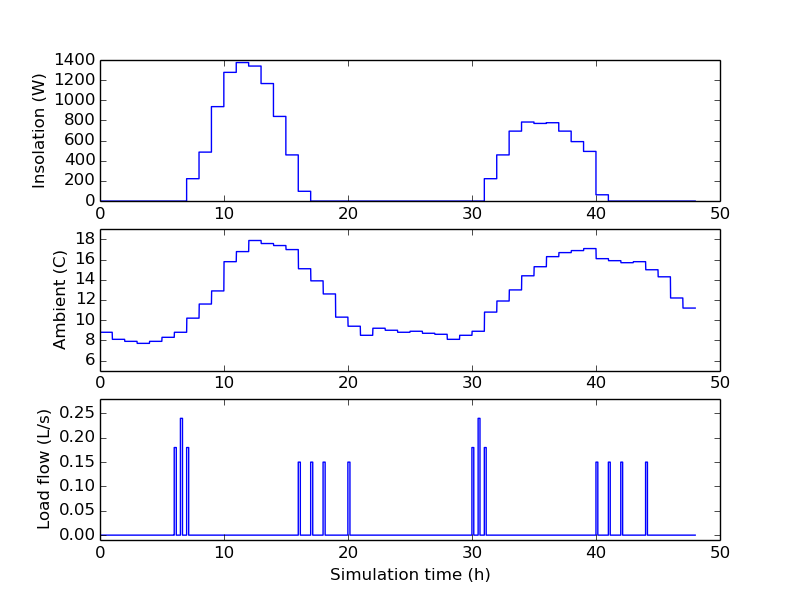
\includegraphics[width=10cm]{images/cer-data}
   \caption{Two days of simulated weather and load conditions}
   \label{fig:cer-data}
\end{figure}

\subsection{Metrics}

The controller's performance was quantified according to three metrics:

\begin{description}
   \item[Satisfaction]
      The user's satisfaction was measured by accumulating the total amounts of time when water was flowing to the user and was at least 50 degrees, and when water was flowing and was less than 50 degrees.
      This number was chosen based on guidelines for domestic water use from Sustainability Victoria~\cite{LSTS}.
   \item[Energy use]
      The total energy use of the controller is integrated across each experiment run.
      This provides an obvious way to compare the strategies of each controller based on how much power they consume to achieve the level of comfort measured by the first metric.
      Note that energy bill is assumed to be implicit in this metric, as this thesis does not take into account the effects of a varying energy price.
   \item[Solar contribution]
      The `solar contribution' refers to the amount of energy gained from sunlight relative to the total amount of energy put into the hot water tank.
      This is a relevant metric as it permits the examination of how effectively the solar resource was exploited.
      However, analysis is complicated by the relationship between solar fraction and total energy used by the controller.
      If one controller expends less control power, all else being equal, it will tend to have a higher solar contribution simply because the amount of energy gained from the sun is now greater in comparison.
      However, this metric does take into account the effect of a tank kept too-hot, which will result in the solar pump differential controller never choosing to let water enter the tank, thereby reducing solar contribution.
\end{description}

These metrics were evaluated each minute during the simulation.

\subsection{Experiment specifications}

\subsubsection{Experiment 1. Comparison to thermostat control}

The goal of this experiment is to compare the predictive controller to the baseline thermostat controller.
For each of the two controllers, eight simulations were run.
Each simulation lasted for one week, and weeks were evenly distributed in December, January, June, and July to compare the operation of the controllers in summer and winter.
It is expected that the predictive controller will have a lower energy usage than the baseline thermostat, but most likely at the cost of some user satisfaction.

\subsubsection{Experiment 2. The effect of inaccurate predictions}

To gauge how critical the effect of prediction accuracy is to the controller's performance, an experiment was set up comparing the controller on a week in july with perfect prediction 9as is standard in all other experiments) and with an incorrect prediction that overestimated how much solar energy would be available.
\Autoref{fig:insolation-error} shows two days from the two profiles used for simulation and prediction.
The predicted profile is identical each day, and overpredicts the amount of insolation.
The true profile is a standard July week.

\begin{figure}
   \centering
   \begin{adjustwidth}{-2cm}{-2cm}
   \begin{subfigure}[b]{0.65\textwidth}
      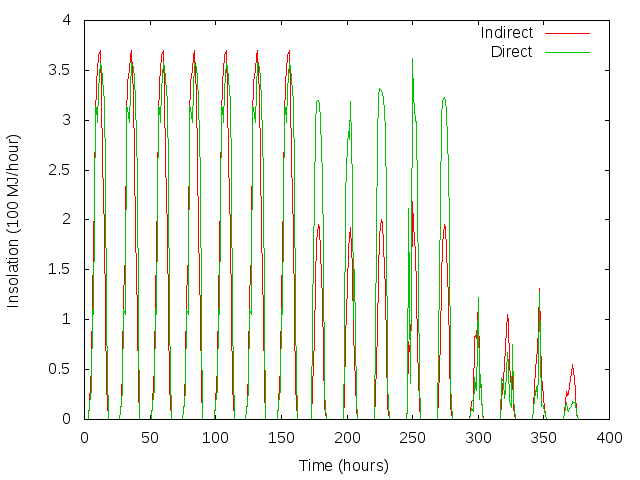
\includegraphics[width=\textwidth]{images/insolation-prediction}
      \caption{Insolation prediction}
      \label{fig:insolation-error-p}
   \end{subfigure}
   ~ %add desired spacing between images, e. g. ~, \quad, \qquad, \hfill etc.
   \begin{subfigure}[b]{0.65\textwidth}
      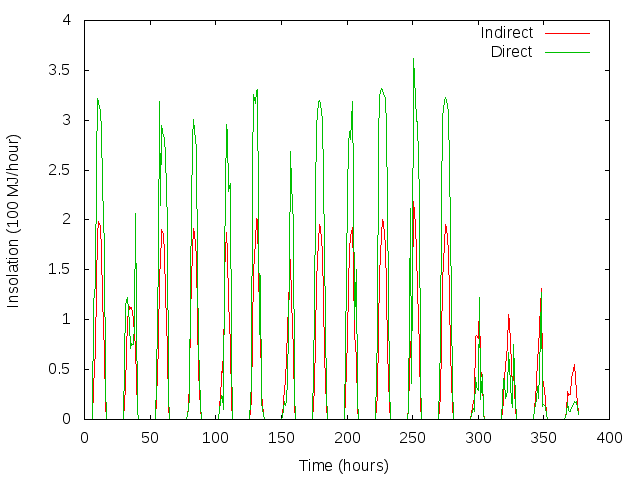
\includegraphics[width=\textwidth]{images/insolation-actual}
      \caption{Actual insolation}
      \label{fig:insolation-error-t}
   \end{subfigure}
   \end{adjustwidth}
   \caption{Insolation profiles for experiment 2}
   \label{fig:insolation-error}
\end{figure}

\subsubsection{Experiment 3. The effect of the control weight}

The controller was designed with a tuning parameter $\rho$ (see \autoref{eq:controller-problem}).
A series of simulations was run with identical conditions except for this parameter.
Eight values were used, arranged linearly from $1\e{-9}$ to $1\e{-5}$.
This was determined to be the range over which the controller varied from maximum satisfaction, keeping the tank very warm most of the time, down to roughly 85\% satisfaction, and only heating the tank immediately before a period of use.

Note that other experiments were conducted with $\rho = 1$.
This provides slightly less comfort and energy usage than the smallest value used in this experiment, and was found to be a good match for thermostat control.

\subsubsection{Experiment 4. The effect of the prediction horizon}

For completeness, it is desirable to determine what effect, if any, the length of the prediction horizon has on the controller's behaviour.
To determine this, a week-long experiment was run five times with controller prediction horizons varying from 4 to 12 hours.
Longer timeframes were not investigated, based on the results achieved from these simulations.

\section{Results}

\begin{figure}
   \centering
   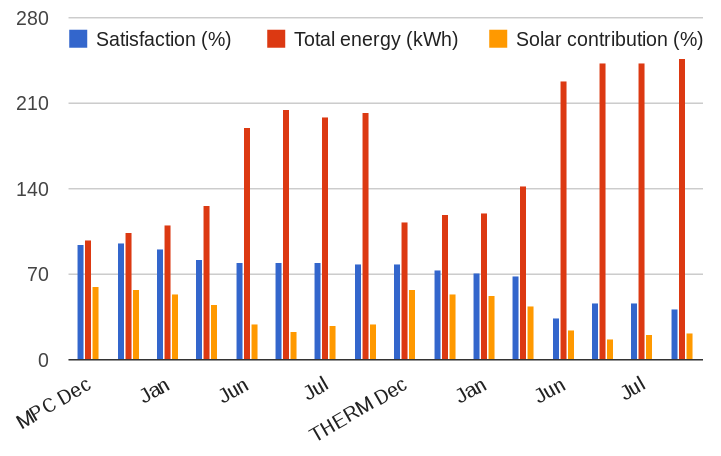
\includegraphics[width=\textwidth]{images/comparison}
   \caption{Comparison of predictive and thermostat control}
   \label{fig:comparison}
\end{figure}

\begin{table}
   \centering
   \begin{tabular}{c c c c}
      Controller & Experiment & Sat (\%) & Energy (kWh) & Solar (\%) \\ \hline
      MPC & Dec 1 & 94.29 & 97.8   & 60.08 \\
          & Dec 2 & 96.19 & 104.1  & 57.19 \\
          & Jan 1 & 91.43 & 110.4  & 54.41 \\
          & Jan 2 & 82.86 & 126.6  & 45.55 \\
          & Jun 1 & 79.37 & 190.2  & 28.99 \\
          & Jun 2 & 79.37 & 205.2  & 23.21 \\
          & Jul 1 & 79.37 & 198.9  & 28.2  \\
          & Jul 2 & 78.73 & 202.5  & 29.38 \\
      THE & Dec 1 & 78.1  & 112.4  & 57.21 \\
          & Dec 2 & 73.97 & 119.5  & 54.32 \\
          & Jan 1 & 71.11 & 120.95 & 53.16 \\
          & Jan 2 & 68.25 & 142.75 & 43.69 \\
          & Jun 1 & 33.97 & 228.05 & 24.27 \\
          & Jun 2 & 46.35 & 243.7  & 17.72 \\
          & Jul 1 & 46.98 & 243.5  & 21.16 \\
          & Jul 2 & 42.22 & 246.35 & 21.78
   \end{tabular}
   \caption{Table of results comparing MPC to thermostat control}
   \label{tab:comparison}
\end{table}

\begin{table}
   \centering
   \begin{tabular}{c c c c}
      $\rho$ & Satisfaction (\%) & Total energy (kWh) & Solar contribution (\%) \\ \hline
      $1\e{-9}$ & 100.00 & 42.90 & 20.39 \\
      $5\e{-9}$ & 100.00 & 42.60 & 20.51 \\
      $1\e{-8}$ & 91.11 & 39.60 & 22.10 \\
      $5\e{-8}$ & 93.33 & 38.70 & 22.52 \\
      $1\e{-7}$ & 91.11 & 38.10 & 22.79 \\
      $5\e{-7}$ & 91.11 & 37.20 & 23.09 \\
      $1\e{-6}$ & 91.11 & 30.30 & 27.23 \\
      $5\e{-6}$ & 84.44 & 25.20 & 31.59 \\
      $1\e{-5}$ & 80.00 & 30.30 & 29.43 \\
   \end{tabular}
   \caption{Table of results comparing tuning values of $\rho$}
   \label{tab:comparison}
\end{table}

\begin{figure}
   \centering
   \begin{adjustwidth}{-2cm}{-2cm}
   \begin{subfigure}[b]{0.65\textwidth}
      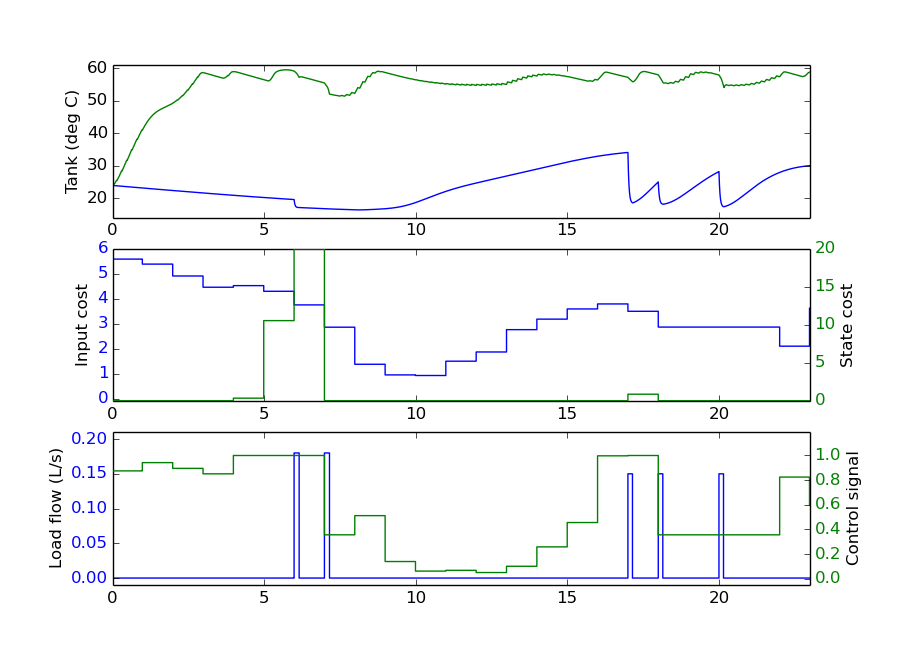
\includegraphics[width=\textwidth]{results/mpc-rho-19}
      \caption{With $\rho = 1\e{-9}$}
      \label{fig:mpc-rho-small}
   \end{subfigure}
   ~ %add desired spacing between images, e. g. ~, \quad, \qquad, \hfill etc.
   \begin{subfigure}[b]{0.65\textwidth}
      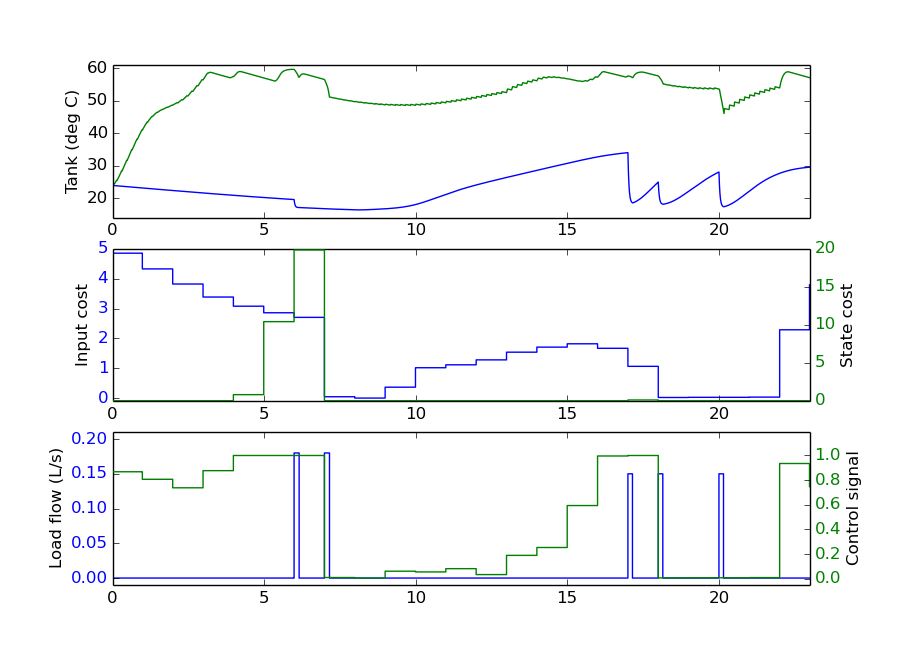
\includegraphics[width=\textwidth]{results/mpc-rho-57}
      \caption{With $\rho = 5\e{-7}$}
      \label{fig:mpc-rho-larger}
   \end{subfigure}
   \end{adjustwidth}
   \caption{Simulations with two values of the tuning parameter $\rho$}
   \label{fig:mpc-rho}
\end{figure}
